\documentclass[10pt, presentation]{beamer}
%[10pt,presentation,german,aspectratio=1610,hyperref={pdfpagemode=FullScreen}]
\usetheme{Madrid}
\usecolortheme{default}
\usepackage[backend=bibtex,style=numeric]{biblatex}
\addbibresource{refs.bib}
\usepackage{graphicx}
\usepackage{multirow}

%\hypersetup{pdfstartview={Fit}}


\title[Machine Learning for DDoS Detection] %optional
{Machine Learning Approaches for Detection of DDoS Attacks in IoT Networks}

\subtitle{}

\author[Adrian Gruszczynski] % (optional, for multiple authors)
{Adrian Gruszczynski}

\institute[Freie Universität Berlin] % (optional)
{
    Institute of Computer Science\\
    Freie Universität Berlin
}

\date[2022] % (optional)
{Seminar IoT \& Security, July 2022}



\AtBeginSection[]
{
    \begin{frame}
        \frametitle{Table of Contents}
        \tableofcontents[currentsection]
    \end{frame}
}

\begin{document}

    \frame{\titlepage}


    \section{Introduction}
%---------------------------------------------------------
    \begin{frame}
        \frametitle{Table of Contents}
        \begin{enumerate}
            \item Introduction
            \item Background
            \begin{enumerate}
                \item Botnets
                \item DDoS
                \item Mirai
                \item Machine Learning 101
            \end{enumerate}
            \item Deep Dive: Malware Detection
            \item Discussion
            \item Conclusion
        \end{enumerate}
    \end{frame}
%---------------------------------------------------------

% Introduciton Motivation
%---------------------------------------------------------
    \begin{frame}
        \frametitle{Introduction}
        \begin{itemize}
            \item Internet of Things is constantly developing
            \begin{itemize}
                \item Estimated 20.4 billion connected devices worldwide in 2022\ \cite{WEBSITE:1}
                \item Applications in various domains e.g.\ smart cities, smart healthcare, autonomous vehicles, industry 4.0, smart grids, etc.
            \end{itemize}
            \item Security and privacy are crucial
            \begin{itemize}
                \item Challenging constrains due to hardware and networking limitations
                \item Heterogeneous networks producing large amounts of data
                \item Low security standards, devices use default credentials \cite{article:8}
            \end{itemize}
            \item Fertile ground for privacy and security attacks
        \end{itemize}
    \end{frame}
%---------------------------------------------------------

% Introduciton DDos
%---------------------------------------------------------
    \begin{frame}
        \frametitle{Introduction}
        \begin{itemize}
            \item Insecure IoT devices may threaten critical Internet infrastructure \cite{article:16}
            \begin{itemize}
                \item Using vulnerable consumer IoT devices becomes a common technique for orchestrating DDoS attacks
                \item Mirai botnet disrupted DNS service of Dyn and significantly limited accessibility of popular services such as Github, Netflix and Amazon
            \end{itemize}
            \item Intelligent system monitoring leveraging ML/DL methods provides a solution for threat detection
            \begin{itemize}
                \item Anomaly detection can facilitate detection of malicious traffic \cite{zargar2013survey}
                \item Prediction of future attacks by learning from existing examples
                \item Malware recognition
            \end{itemize}
        \end{itemize}
    \end{frame}

%---------------------------------------------------------


    \section{Background}

% Botnets
%---------------------------------------------------------
    \begin{frame}
        \frametitle{Botnets}
        \begin{itemize}
            \item Group of devices infected by malware
            \item The size varies from hundreds to hundreds of thousands of devices \cite{article:8}
            \item Can be controlled remotely by an attacker to execute malicious activities
            \begin{itemize}
                \item Phishing
                \item Spamming
                \item DDoS
            \end{itemize}
            \item IoT provides an ideal foundation for botnets and carrying out DDoS attacks
            \begin{itemize}
                \item Easy target due to low security measures in IoT
                \item High number of hackable devices
                \item Massive pool of legitimate IP addresses and sources of traffic
            \end{itemize}
        \end{itemize}
    \end{frame}

% DDoS
%---------------------------------------------------------
    \begin{frame}
        \frametitle{DDoS}
        \begin{itemize}
            \item Cyberattack that targets a host, network or infrastructure \cite{article:8}
            \item The goal is to render the target unavailable for others by exhausting its resources (Bandwidth, Memory, CPU, etc.)
            \item Attacks on critical internet infrastructure (DNS) have an enormous impact
            \item Thanks to the broad availability of botnets DDoS is a simple yet powerful weapon
            \item DDoS attacks happen on two levels:
            \begin{itemize}
                % Dont finish 3 way handshake or send a packet with origin IP adress same as receiving to crash the server
                \item Network-level: exploits network layer protocols e.g.\ TCP, UDP, IP, etc.
                % Send POST request very slowly or request
                \item Application-level: exploits application layer protocols e.g.\ HTTP, DNS, etc.
            \end{itemize}
            \item There is a number of DDoS techniques including:
            \begin{itemize}
                % Dont finish 3 way handshake or send a packet with origin IP adress same as receiving to crash the server
                \item Amplification: generate most traffic with least amount of bandwidth
                % Send POST request very slowly or request
                \item Reflection: used in combination with IP-spoofing to hide the origin IP
            \end{itemize}
        \end{itemize}
    \end{frame}

%---------------------------------------------------------

% Mirai botnet
%---------------------------------------------------------
%    \begin{frame}
%        \frametitle{Mirai}
%        \begin{itemize}
%            % Embed figure 5 from 7178164.pdf
%            \item DDoS capable malware that first appeared in 2016
%            \item Responsible for the biggest scale DDoS attack ever recorded peaking at 1.2Tbps \cite{article:8}
%            \begin{itemize}
%                \item Rendered popular internet services unavailable (Github, Netflix, Amazon, etc.)
%                \item Impacted United States and Europe
%            \end{itemize}
%            \item Botnet of approximately 500k compromised devices
%            \item Source code was published causing a number of similar attacks to follow
%        \end{itemize}
%    \end{frame}

% Mirai figure
% TODO: Figure doesn't scale
%---------------------------------------------------------
    \begin{frame}
        \frametitle{Mirai - logical infrastructure}
        \begin{columns}
            \column{0.5\textwidth}
            \begin{itemize}
                % Embed figure 5 from 7178164.pdf
                \item DDoS capable malware that first appeared in 2016
                \item Responsible for the biggest scale DDoS attack ever recorded peaking at 1.2Tbps \cite{article:8}
                \begin{itemize}
                    \item Rendered popular internet services unavailable (Github, Netflix, Amazon, etc.)
                    \item Impacted United States and Europe
                \end{itemize}
                \item Botnet of approximately 500k compromised devices
                \item Source code was published causing a number of similar attacks to follow
            \end{itemize}
            \column{0.5\textwidth}
            \begin{figure}
                \centerline{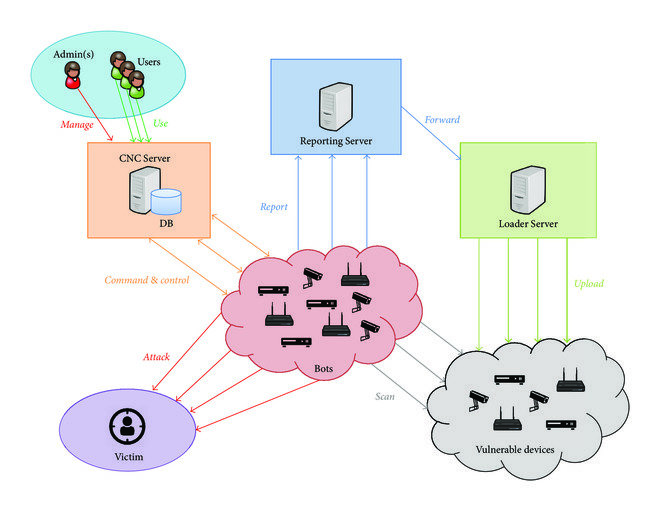
\includegraphics[scale=0.28,keepaspectratio]{figures/Mirai-logical-infrastructure.png}}
                \caption{Mirai logical infrastructure \cite{article:8}}
            \end{figure}
        \end{columns}


    \end{frame}

    \begin{frame}
        \frametitle{Machine learning 101 - Basics}
        \begin{columns}
            \column{0.5\textwidth}
            \begin{itemize}
                \item Allows for solving of complex problems without a predefined set of rules \cite{Goodfellow-et-al-2016}
                \item Tasks include classification, anomaly detection and translation
                \item Classification based on training approach:
                \begin{itemize}
                    \item Supervised: requires pairs of input x and output y, want to learn mapping from x to y  (classification, regression)
                    \item Unsupervised: uses unlabelled data to extract latent patterns (clustering, denoising, compression)
                \end{itemize}
            \end{itemize}
            \column{0.5\textwidth}
            \begin{figure}
                \centerline{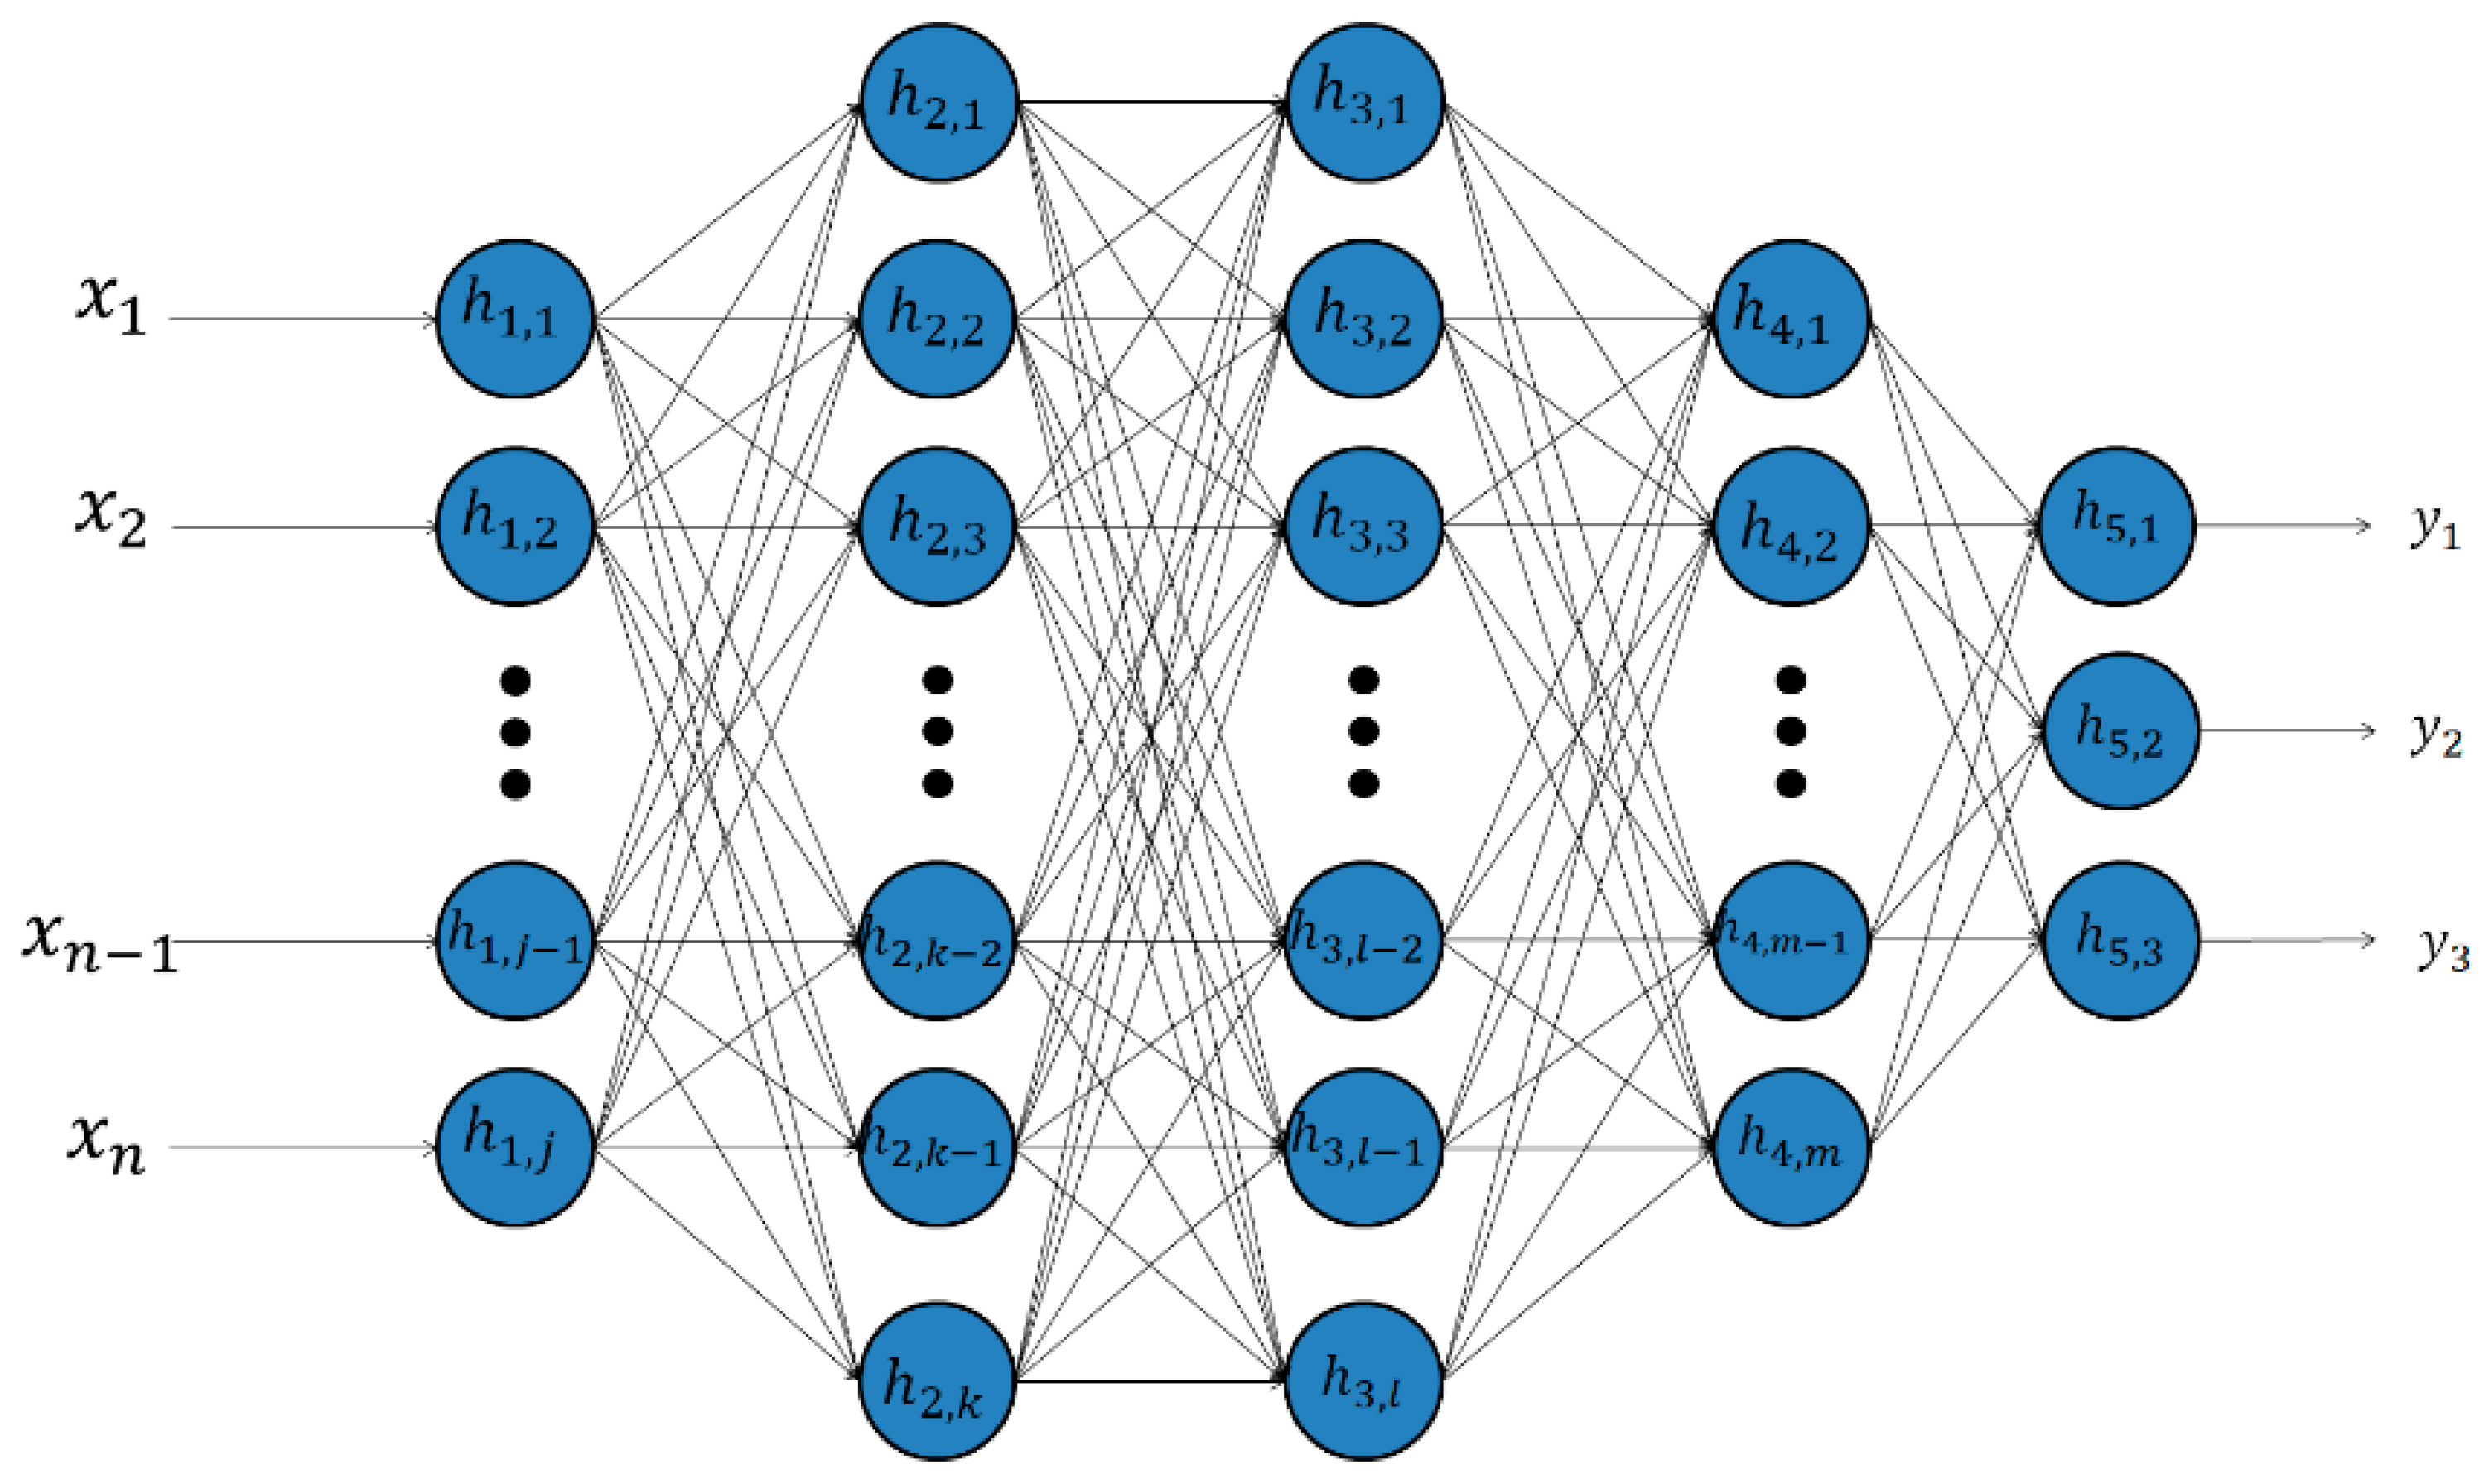
\includegraphics[scale=0.06,keepaspectratio]{figures/ann.jpg}}
                \caption{Visual representation of a feed forward neural network \cite{article:18}.}
            \end{figure}
        \end{columns}
    \end{frame}

    \begin{frame}
        \frametitle{Machine learning 101 - Optimisation}
        \begin{columns}
            \column{0.5\textwidth}
            \begin{itemize}
                \item Dataset divided into training and test part
                \item Model sees the entire training data example by example and tries to predict the output given an input
                \item It learns the dependencies by adjusting its internal parameters to minimise the prediction error
                \item The learning takes place using stochastic gradient descent and backpropagation
                \item After training models gets evaluated with the test data to assess real performance on unseen data
            \end{itemize}
            \column{0.5\textwidth}
            \begin{figure}
                \centerline{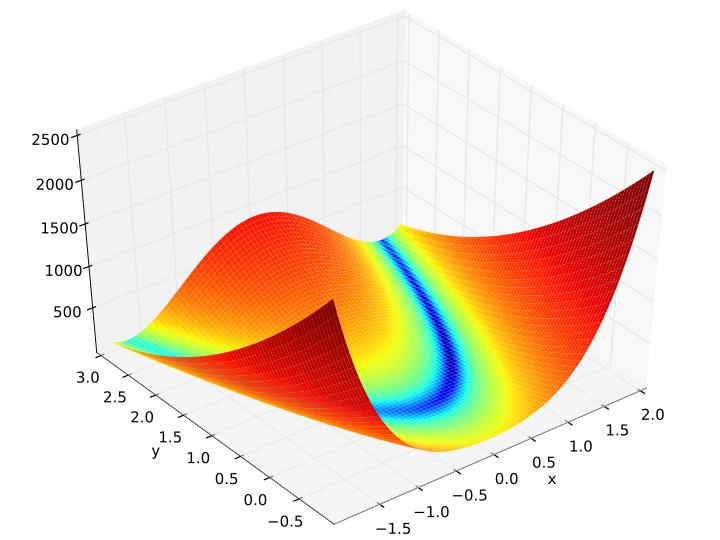
\includegraphics[scale=0.28,keepaspectratio]{figures/loss_landscape.png}}
                \caption{Visual representation of a 2D loss landscape \cite{Goodfellow-et-al-2016}.}
            \end{figure}
        \end{columns}
    \end{frame}

    \begin{frame}
        \frametitle{Machine learning 101 - Performance Measures}
        \begin{columns}
            \column{0.5\textwidth}
            \begin{itemize}
                \item Performance of a model depends on a problem
                \item Accuracy for classification: ratio of correctly predicted examples to all predicted
                \item Mean Squared Error (MSE) for regression tasks
                \item For unsupervised tasks performance metrics are problem dependent
            \end{itemize}
            \column{0.5\textwidth}
            \begin{table}[htbp]
                \begin{tabular}{l|l|c|c|c}
                    \multicolumn{2}{c}{} & \multicolumn{2}{c}{$y$} & \\
                    \cline{3-4}
                    \multicolumn{2}{c|}{} & Positive & Negative & \multicolumn{1}{c}{} \\
                    \cline{2-4}
                    \multirow{2}{*}{$\hat{y}$} & Positvive                 & $a$                       & $b$                       & $$                   \\
                    \cline{2-4}
                    & Negative                  & $c$                       & $d$                       & $$                   \\
                    \cline{2-4}
                    \multicolumn{1}{c}{}       & \multicolumn{1}{c}{Total} & \multicolumn{1}{c}{$a+c$} & \multicolumn{    1}{c}{$$} & \multicolumn{1}{c}{$$}\\
                \end{tabular}
                \caption{Confusion matrix.}
                \label{tab:cm}
            \end{table}
        \end{columns}
    \end{frame}





    \section{Deep Dive}

% ConvNets
% TODO: Figure doesn't fit
%---------------------------------------------------------
    \begin{frame}
        \frametitle{Convolutional Neural Network}
        \begin{itemize}
            \item Ability to learn complex spatial dependencies in image data \cite{Goodfellow-et-al-2016}
            \item Builds its own understanding of images by extracting high level feature representations
            \item Architecture is a combination of convolutional and pooling layers
            \begin{itemize}
                \item Convolution works by shifting a filter through the input and computing a dot product
                \item Pooling is a nonlinear down sampling of the input to reduce amount of information
            \end{itemize}
            \item Broad range of application in image recognition, image segmentation, speech recognition, anomaly detection, etc.
        \end{itemize}
        \begin{figure}
            \centerline{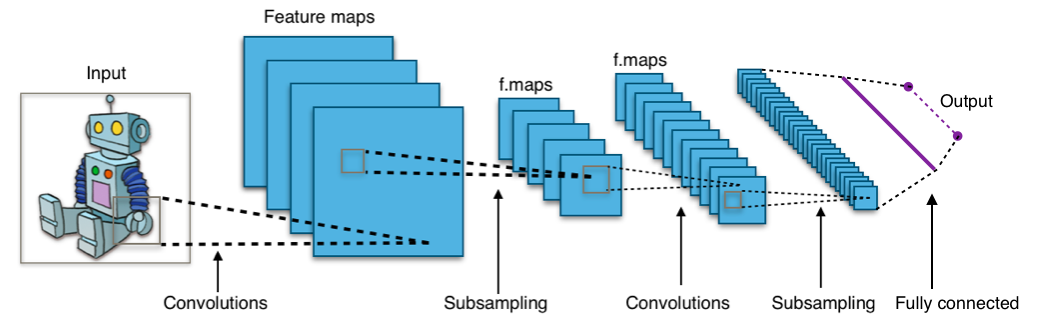
\includegraphics[width=\linewidth,height=0.3\textheight,keepaspectratio]{figures/cnn2.png}}
            \caption{Convolutional neural network: visual representation \cite{WEBSITE:1}.}
        \end{figure}
    \end{frame}

% Malware detection study
%---------------------------------------------------------
    \begin{frame}
        \frametitle{Malware Detection Using Image Recognition}
        \begin{itemize}
            \item Researchers visualised malware binaries as grayscale images \cite{article:3}
            \item They used the images in combination with image recognition techniques for malware detection
            \item One study uses a convolutional neural network to classify images a malware or goodware based
            \item They use IoTPOT \cite{IoTPOT} data that has examples of malware binaries from two families: Mirai and Gafgyt
            \item The authors propose a 2-tier architecture
            \begin{itemize}
                \item Lightweight convolutional neural network that runs on the IoT device
                \item The device can detect suspicious software with roughly 94\% accuracy
                \item Software classified as malware gets sent to the cloud for further examination
            \end{itemize}
        \end{itemize}
        \begin{figure}
            \centerline{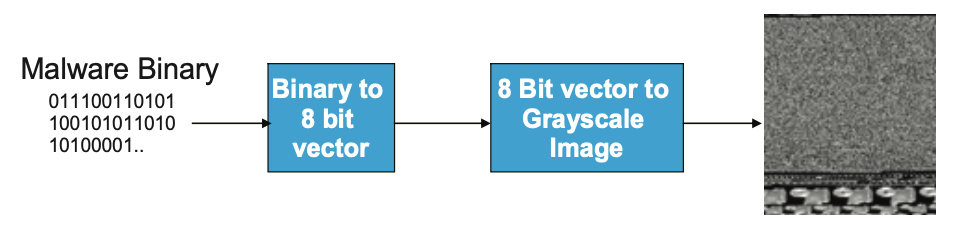
\includegraphics[width=\linewidth,height=0.25\textheight,keepaspectratio]{figures/malware-to-gray.png}}
            \caption{Visualising malware as 8-bit grayscale images \cite{article:7}.}
        \end{figure}

    \end{frame}


    \section{Discussion and Conclusion}

% Discussion
%---------------------------------------------------------
    \begin{frame}
        \frametitle{Discussion}
        \begin{itemize}
            \item Authors show that on-device deep learning is a feasible approach
            \item The proposed method is vulnerable to obfuscation and encryption
            \item It is questionable how well this generalizes to new malware families
            \item Models have to be re-trained and re-distributed
            \item In contrast to network-based DDoS detection this method requires tampering with devices
        \end{itemize}
    \end{frame}

% Conclusion
%---------------------------------------------------------
    \begin{frame}
        \frametitle{Conclusion}
        \begin{itemize}
            \item Machine and deep learning show great potential for anomaly and malware detection \cite{Goodfellow-et-al-2016}
            \item Deep learning methods enable learning complex patterns without manual feature engineering \cite{Goodfellow-et-al-2016}
            \item The researchers use data of DDoS traffic simulated in a lab environment \cite{article:4}, \cite{inproceedings:1}
            \begin{itemize}
                \item Difficult to compare results
                \item Questionable real life performance
            \end{itemize}
            \item Low availability of public datasets for DDoS and DDoS malware detection
            \item Methods that detect unknown attacks show high potential \cite{article:4}
            \item On-device anomaly and malware detection is not well researched yet
            \item Regulatory approaches seem promising in long term \cite{article:12}
            \item Ease of integration into existing systems plays key role \cite{inproceedings:1}
            \item Future research should focus on transfer learning, autoencoders and unsupervised learning
        \end{itemize}
    \end{frame}

%Refs
%---------------------------------------------------------
    \begin{frame}
        \frametitle{References}
        \printbibliography
    \end{frame}

\end{document}